\documentclass{sigchi}

% Use this section to set the ACM copyright statement (e.g. for
% preprints).  Consult the conference website for the camera-ready
% copyright statement.

% Copyright
\CopyrightYear{2020}
%\setcopyright{acmcopyright}
\setcopyright{acmlicensed}
%\setcopyright{rightsretained}
%\setcopyright{usgov}
%\setcopyright{usgovmixed}
%\setcopyright{cagov}
%\setcopyright{cagovmixed}
% DOI
\doi{https://doi.org/10.1145/3313831.XXXXXXX}
% ISBN
\isbn{978-1-4503-6708-0/20/04}
%Conference
\conferenceinfo{CHI'20,}{April  25--30, 2020, Honolulu, HI, USA}
%Price
\acmPrice{\$15.00}

% Use this command to override the default ACM copyright statement
% (e.g. for preprints).  Consult the conference website for the
% camera-ready copyright statement.

%% HOW TO OVERRIDE THE DEFAULT COPYRIGHT STRIP --
%% Please note you need to make sure the copy for your specific
%% license is used here!
% \toappear{
% Permission to make digital or hard copies of all or part of this work
% for personal or classroom use is granted without fee provided that
% copies are not made or distributed for profit or commercial advantage
% and that copies bear this notice and the full citation on the first
% page. Copyrights for components of this work owned by others than ACM
% must be honored. Abstracting with credit is permitted. To copy
% otherwise, or republish, to post on servers or to redistribute to
% lists, requires prior specific permission and/or a fee. Request
% permissions from \href{mailto:Permissions@acm.org}{Permissions@acm.org}. \\
% \emph{CHI '16},  May 07--12, 2016, San Jose, CA, USA \\
% ACM xxx-x-xxxx-xxxx-x/xx/xx\ldots \$15.00 \\
% DOI: \url{http://dx.doi.org/xx.xxxx/xxxxxxx.xxxxxxx}
% }

% Arabic page numbers for submission.  Remove this line to eliminate
% page numbers for the camera ready copy
% \pagenumbering{arabic}

% Load basic packages
\usepackage{balance}       % to better equalize the last page
\usepackage{graphics}      % for EPS, load graphicx instead 
\usepackage[T1]{fontenc}   % for umlauts and other diaeresis
\usepackage{txfonts}
\usepackage{mathptmx}
\usepackage[pdflang={en-US},pdftex]{hyperref}
\usepackage{color}
\usepackage{booktabs}
\usepackage{textcomp}

% Some optional stuff you might like/need.
\usepackage{microtype}        % Improved Tracking and Kerning
% \usepackage[all]{hypcap}    % Fixes bug in hyperref caption linking
\usepackage{ccicons}          % Cite your images correctly!
% \usepackage[utf8]{inputenc} % for a UTF8 editor only

% If you want to use todo notes, marginpars etc. during creation of
% your draft document, you have to enable the "chi_draft" option for
% the document class. To do this, change the very first line to:
% "\documentclass[chi_draft]{sigchi}". You can then place todo notes
% by using the "\todo{...}"  command. Make sure to disable the draft
% option again before submitting your final document.
\usepackage{todonotes}

%
\usepackage{gensymb}
\usepackage{array}
\newcolumntype{C}[1]{>{\centering\arraybackslash}p{#1}}
%

% Paper metadata (use plain text, for PDF inclusion and later
% re-using, if desired).  Use \emtpyauthor when submitting for review
% so you remain anonymous.
\def\plaintitle{CollaboVR: A Reconfigurable Framework for Multi-user to Communicate in Virtual Reality}
\def\plainauthor{Zhenyi He, Ken Perlin}
\def\emptyauthor{}
\def\plainkeywords{Virtual Reality; freehand drawing; computer-supported collaborative work.}
\def\plaingeneralterms{Documentation, Standardization}

% llt: Define a global style for URLs, rather that the default one
\makeatletter
\def\url@leostyle{%
  \@ifundefined{selectfont}{
    \def\UrlFont{\sf}
  }{
    \def\UrlFont{\small\bf\ttfamily}
  }}
\makeatother
\urlstyle{leo}

% To make various LaTeX processors do the right thing with page size.
\def\pprw{8.5in}
\def\pprh{11in}
\special{papersize=\pprw,\pprh}
\setlength{\paperwidth}{\pprw}
\setlength{\paperheight}{\pprh}
\setlength{\pdfpagewidth}{\pprw}
\setlength{\pdfpageheight}{\pprh}

% Make sure hyperref comes last of your loaded packages, to give it a
% fighting chance of not being over-written, since its job is to
% redefine many LaTeX commands.
\definecolor{linkColor}{RGB}{6,125,233}
\hypersetup{%
  pdftitle={\plaintitle},
% Use \plainauthor for final version.
%  pdfauthor={\plainauthor},
  pdfauthor={\emptyauthor},
  pdfkeywords={\plainkeywords},
  pdfdisplaydoctitle=true, % For Accessibility
  bookmarksnumbered,
  pdfstartview={FitH},
  colorlinks,
  citecolor=black,
  filecolor=black,
  linkcolor=black,
  urlcolor=linkColor,
  breaklinks=true,
  hypertexnames=false
}

% create a shortcut to typeset table headings
% \newcommand\tabhead[1]{\small\textbf{#1}}

% End of preamble. Here it comes the document.
\begin{document}

\title{\plaintitle}

\numberofauthors{3}
\author{%
  \alignauthor{Leave Authors Anonymous\\
    \affaddr{for Submission}\\
    \affaddr{City, Country}\\
    \email{e-mail address}}\\
  \alignauthor{Leave Authors Anonymous\\
    \affaddr{for Submission}\\
    \affaddr{City, Country}\\
    \email{e-mail address}}\\
  \alignauthor{Leave Authors Anonymous\\
    \affaddr{for Submission}\\
    \affaddr{City, Country}\\
    \email{e-mail address}}\\
}

\teaser{
%\begin{subfigure}
    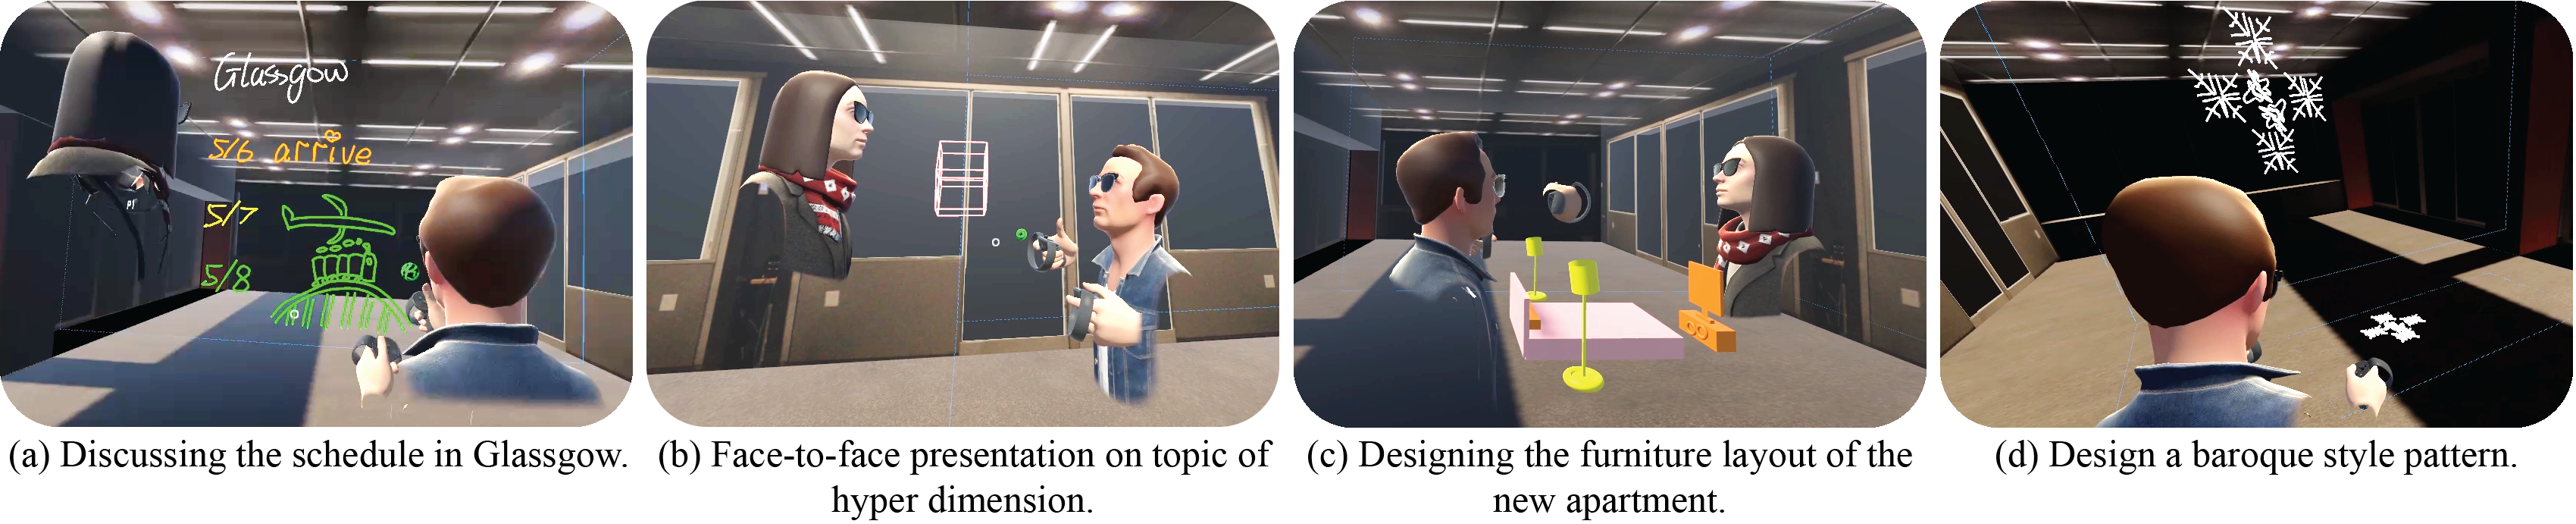
\includegraphics[width=0.85\paperwidth]{Figure1.png}
%\end{subfigure}
\caption{CollaboVR is a reconfigurable framework for multi-user communication in Virtual Reality. Here are four use cases of CollaboVR. Figure (a) demonstrates how people use it to schedule daily life. Figure (b) demonstrates a face-to-face presentation on the topic of hyper dimension. Figure (c) illustrates how to discuss furniture placement with a roommate. Figure (d) illustrates a person learning baroque style design. Different combinations of \textit{user arrangement} and \textit{input orientation} are applied to the above user cases for better communication effects.}
\label{fig:teaser}
} %using an entire image for final version
 
\maketitle

\begin{abstract}
  Despite various collaborative software that supports expressing ideas, people still largely prefer physical notebooks or whiteboards. The reason is that they provide free-form expressions, co-presence of all participants and easy collaboration. However, when working with remote participants, people often choose the convenience of video conferencing, perhaps with screen sharing. We propose CollaboVR, an open-source reconfigurable framework for distributed and co-located multi-user communication in Virtual Reality. We tested CollaboVR with an application that lets participants create freehand drawings and 3D objects, while allowing participants to adjust two key variables: (1) User arrangement (participants adjust the location of their views of other participants) and (2) Input orientation (participants adjust the input to be vertical or horizontal). Preliminary user studies show that CollaboVR is a useful collaborative tool. Users report that some user arrangements and input orientations work best for brainstorming, while others work best for presentation or collaborative refinement of designs.
\end{abstract}


% ACM Classfication

\begin{CCSXML}
<ccs2012>
<concept>
<concept_id>10003120.10003121.10003124.10010866</concept_id>
<concept_desc>Human-centered computing~Virtual reality</concept_desc>
<concept_significance>500</concept_significance>
</concept>
<concept>
<concept_id>10003120.10003121.10003124.10011751</concept_id>
<concept_desc>Human-centered computing~Collaborative interaction</concept_desc>
<concept_significance>500</concept_significance>
</concept>
</ccs2012>
\end{CCSXML}

\ccsdesc[500]{Human-centered computing~Virtual reality}
\ccsdesc[500]{Human-centered computing~Collaborative interaction}

% Author Keywords
\keywords{\plainkeywords}

% Print the classficiation codes
%\printccsdesc
%Please use the 2012 Classifiers and see this link to embed them in the text: \url{https://dl.acm.org/ccs/ccs_flat.cfm}



\section{Introduction}
% VR for workspace and collaboration, however the communication layer still remain the same for most of them
% communication work. Workspace awareness is one important key. -- user arrangement design
% Inspired by taxomony and other tabletop work, we proposed ... a reconfigurable ... to see how mid-air visual aids work and how the two vars affect the experience
% List all the contributions
Virtual Reality (VR) is increasingly being explored as a tool for human-computer interaction (HCI), spurred by the availability of high quality consumer headsets in recent years. VR enables a rich design space in HCI by providing 3D input and immersive experiences. In 1998, the "Office of the future"~\cite{raskar1998office}, was proposed to allow remotely located people to feel as though they were together in a shared office space, via a hybrid of modalities including telepresence, large panoramic displays and manipulation of shared 3D objects. The core idea was that VR had the potential to enhance communication and collaboration among groups of people, as well as Augmented Reality (AR) and projection-based immersive experiences. Since then, significant progress has been made in exploring techniques for communication~\cite{ishii1993integration, otsuka2016mmspace}, collaborative works~\cite{kunert2014photoportals,tang2010three}, infrastructure~\cite{maimone2013general, o2011blended, thomas2014muvr} and various modalities~\cite{follmer2013inform, leithinger2014physical, leithinger2015shape, nakagaki2019inforce} in the field of multi-user experiences. However, we found that many works are still using mono audio as the only direct communication method during immersive collaborative experiences~\cite{xia2018spacetime}, and others provide only indirect communication approaches such as changing the color of a shared target~\cite{huo2018synchronizar}. In this paper, we consider designing a VR communication framework that could be potentially beneficial to various collaborative experiences.

% How other ppl contribute to related area, communication/collaboration/co-located and distributed
Much research has contributed to improving communication through VR, AR or tabletop interfaces for both co-located and distributed groups. As observed by Lindemann ~\cite{tversky2003human}, gestures or visual aids are commonly used while speaking to others in daily life. Awareness of these behaviors is technically considered as \textit{workspace awareness}, defined as the up-to-the-moment understanding of other people's interaction in a shared workspace~\cite{li2014interactive}. Providing workspace awareness is widely employed in many research studies. 
%Prior work tried to improve communication using alternative arrangements of spaces and enhanced digital content for communication. 
One trend is improving communication through shared display. Some work enables face-to-face interaction, such as VideoDraw~\cite{tang1990videodraw}, ClearBoard~\cite{ishii1993integration} and FacingBoard~\cite{li2014interactive}. More traditional techniques, including white-boards and side-by-side projected displays, have been shown to improve group performance as well~\cite{plaue2009presence}. Furthermore, MMSpace implemented kinetic displays so that each display can change its orientation to realize face-to-face interaction for different participants~\cite{otsuka2016mmspace}.
Another trend is the use of tabletop tangible devices~\cite{brave1998tangible, kunert2019multi}, which also enhance co-presence of other people in the group. Inspired by this previous work, we propose to design a multi-user system which supports different options for user arrangement (the ways that participants can adjust the views of other participants) and input orientation (the ways that participants can adjust the orientation of the input surface).

We propose CollaboVR, an open-source reconfigurable framework for distributed and co-located multi-user communication in VR. The framework includes the following:
\begin{itemize}
    \item A protocol connecting the application to the VR clients. To provide rich and smart visual aids, we choose Chalktalk, an open-source digital presentation and communication language to support freehand drawing and 3D objects~\cite{perlin2018chalktalk}. More details are described later.
    \item A star network to support communication between distributed clients and the server.
    \item Rich interactions for manipulating drawings so that all of the visual aids (freehand drawing or 3D objects) can be further manipulated after being drawn.
    \item Multiple user arrangements in which participants can adjust the location of their views of other participants.
    \item Multiple input orientations in which participants can adjust the vertical versus horizontal angle of the input area.
\end{itemize}

Our main contributions in this paper are as follows:
\begin{enumerate}
    \item Designing and implementing an open-source reconfigurable framework for multi-user communication. The code will be made available \url{masked For Anonymity}.
    \item A system evaluation which indicates that CollaboVR is a useful multi-user tool in terms of communication.
    \item Qualitative feedback which indicates that different combinations of two key variables (user arrangement and input orientation) function differently for different collaborative purposes.
\end{enumerate}

%\section{Scenario[opt]}

\section{Related Work}
% not smooth
CollaboVR is a framework to assist communication. By definition, communication is the act of expressing and understanding among a group. Similarly, \textit{sensemaking} is the understanding of the meaning of a communicative act~\cite{paul2009understanding}. Sensemaking is a widely researched concept in the area of information visualization. Dervin describes sensemaking as using ideas, emotions and memories to bridge a gap in understanding in a group~\cite{dervin1992mind}. Learning how collaborative sensemaking is supported through different design considerations is very useful for multi-user communication. In this section, we introduce collaborative sensemaking approaches first. Second, we summarize that how workspace awareness has positive effects on collaboration and how previous studies enhance workspace awareness. Last, we introduce immersive collaboration and communication and assess their advantages and limitations.

\subsection{Collaborative Sensemaking}
%introduce the definition of sensemaking somewhere and how we deal with it
Many previous works have researched sensemaking in different domains in HCI and computer-supported collaborative work (CSCW) area~\cite{albolino2007sensemaking, billman2007medical, landgren2007study,paul2009understanding}. Given that sensemaking involves data analysis~\cite{yi2008understanding}, different designs of 2D displays and digital tabletop are frequently discussed. Prior work has shown two things: First, large and shared displays have been shown to benefit sensemaking groups in several contexts. Sharodal designed CoSense~\cite{dervin1992mind} with a shared display, conducted an ethnographic study, and examined how collaborative sensemaking can be supported. Vogt et al. found that the large display facilitated the paired sensemaking process, allowing teams to spatially arrange information and conduct individual work as needed~\cite{vogt2011co}. Moreover, multiple digital tabletops were used for sensemaking tasks ~\cite{isenberg2010exploratory,morris2010wesearch}. Second, personal displays may lead to decreased collaboration in co-located settings ~\cite{chung2013investigating, wallace2009investigating}.
When designing CollaboVR, we considered the idea of "multiple" displays, displays with "different" angles, as well as adding "personal" displays into the mix, which leads to the design of different input orientations and the placement of visual aids.

\subsection{Workspace Awareness}
Workspace awareness is the collection of up-to-the-minute knowledge a participant has of other participants' interaction with the workspace~\cite{gutwin1996workspace}. It includes the awareness of others' locations, activities, and intentions relative to the task and to the space. Maintaining workspace awareness enables participants to work together more effectively~\cite{gutwin1998design, gutwin2002descriptive}. Workspace awareness plays an important role in simplifying communication, taking turns and action prediction ~\cite{gutwin2002descriptive}. In brief, maintaining and enhancing workspace awareness is beneficial to collaboration. 

One trend is the use of see-through displays for distributed collaboration. The idea started with Tang and Minneman, who designed VideoDraw~\cite{tang1990videodraw} and VideoWhiteBoard~\cite{tang1991videowhiteboard}. Both approaches are two-user experiences. On each side, a video camera was placed to capture the local user and the drawing. A projector was attached to present the remote user and the drawing on the top of the local display. ClearBoard~\cite{ishii1992clearboard} extended the idea and used digital media. Instead of using projectors, the media displayed the video feed of the remote user and drawing to maintain workspace awareness. Similarly, KinectArms~\cite{genest2013kinectarms} used a tangible tabletop as the media, and rendered the arm of the remote user for mixed presence. Furthermore, Jiannan et al.~\cite{li2014interactive} developed FacingBoard with two-sided transparent displays. Analogous to ClearBoard, the entire upper-body is displayed to the other participants so that gaze awareness is supported. To maintain gaze interaction, FacingBoard reversed the graphics on the display. However, some column-sensitive content, such as text and map then became incorrect. To solve this problem, FacingBoard selectively flipped the column-sensitive content individually and adjusted the position of the content. However, when people pinpointed a specific sub-area within the content, the gaze and the place being pinpointed were inconsistent to both users. In our system, we proposed different user arrangements to enhance workspace awareness. We also provide a similar face-to-face experience. Differently, we manipulate the users' locations to maintain gaze awareness rather than flipping the content, and we support collaboration between more than two people. This is detailed later.

\subsection{Immersive Collaboration and Communication}
% we need more and more because reviews were complaining the amount
% think about the trend
Much work has been done in collaborative applications in VR and mixed reality (MR). Some has focused on multi-user gaming experiences. SynchronizAR designed a registration algorithm for mobile AR so that participants could join the co-located experience without needing to take extra steps to ensure high-quality positional tracking~\cite{huo2018synchronizar}.
Some has focused on developing telepresence experiences and bridging the gap between the physical and virtual worlds. InForce created a set of novel interaction techniques, including haptic feedback for distributed collaboration ~\cite{nakagaki2019inforce}.
MetaSpace performed full body tracking for distributed users to create a sense of presence~\cite{sra2015metaspace}.
Holoportation demonstrated 3D reconstructions of an entire space including reconstruction of people~\cite{orts2016holoportation}.
Immersive group-to-group telepresence allowed distributed groups of users to meet in a shared virtual 3D world through two coupled projection-based setups~\cite{beck2013immersive}. Depth and color cameras were used for reconstruction. Some designed a collaborative tool for productive work, such as editing and modeling. SpaceTime focused on improving the experience for two experts collaborating on design work together~\cite{xia2018spacetime}. It designed "parallel objects" to resolve interaction conflicts and to support design workflows. Some put more effort in object manipulation and navigation. T(ether) is a spatially aware display system for co-located collaborative manipulation and animation of objects ~\cite{lakatos2014t}. Trackable markers on pads and digital gloves allow participants to manipulate objects in space through gestures. Andre et al. designed an application to support object manipulation tasks and scene navigation from different views ~\cite{kunert2019multi}. Some developed a distributed system for remote assistance. Virtual Replicas for Remote Assistance is a remote collaboration system allowing a remote expert to guide local users to assemble machine parts by using virtual replicas~\cite{oda2015virtual}. Others such as Geollery~\cite{du2019geollery, du2016social} focused on social experiences among users, by creating and the studying an interactive MR social media platform.

For collaborative purposes such as social networking and telepresence, engagement and a sense of being there are the most important qualities. In those scenarios, communication performance is not the focus. While for collaborative purposes, such as productive work, games, assistance or object manipulation, which require complicated and specific operations and information exchange during the process of collaboration, communication performance becomes more important. Our goal is to build a reconfigurable framework to fit different purposes of collaboration.

% fill with old submission and go through chi+cscw+uist for recent 5 years.
Next, we examine the trending of communication in immersive environments. Some have proposed asymmetrical communication. ShareVR enables communication between an HMD user and a non-HMD user~\cite{gugenheimer2017sharevr}. By using floor projection and mobile displays to visualize the virtual world, the non-HMD user can interact with the HMD user and become part of the VR experience. Mutual human actuation~\cite{cheng2017mutual} runs pairs of users at the same time and has them provide human actuation to each other. Communication between the pair is through shared interactive props.

Interacting with digital content in a shared space is also common. Three's Company~\cite{tang2010three} explored the design of a system for three-way collaboration over a shared visual workspace. They illustrated the utility of multiple configurations of users around a distributed workspace. TwinSpace supports deep interconnectivity and flexible mappings between virtual and physical spaces~\cite{reilly2010twinspace}. Your Place and Mine explored three ways of mapping two differently sized physical spaces to shared virtual spaces to understand how social presence, togetherness, and movement are influenced~\cite{sra2018}. Tan et al. built a face-to-face presentation system for remote audiences ~\cite{gazeAwareness}. Tele-Board~\cite{gumienny2011tele} designed a groupware system focused on creative working modes using a traditional whiteboard and sticky notes in digital form for distributed users. Hrvoje Benko et al. proposed a unique spatial AR system that enables two users to interact with a shared virtual scene and each other in a face to face arrangement~\cite{benko2014dyadic}. We found that much work focused on two-user or pair communication. Our work proposes a solution to scale the number of participants. In addition, we have observed that many studies have experimented with a face-to-face setup with shared display or a round table for communication. We propose two variances: variance in user arrangement and variance in input orientation, to investigate their respective advantages and limitations.

\section{CollaboVR Overview}
In this section, we present an overview of CollaboVR's system architecture. CollaboVR consists, essentially, of a protocol that serializes input and display data from each user of an application, routes that data through a network, and then de-serializes and interprets the data to correctly render the results into graphics. Currently, we have tested CollaboVR with the application Chalktalk~\cite{perlin2018chalktalk}. Chalktalk is an open-source digital presentation and communication language. It allows a presenter to create and interact with animated digital sketches on a blackboard-like interface. There are some other smart sketch-based online software programs, such as Autodraw~\cite{Autodraw}, sketch2code~\cite{Sketch2code} and Miro~\cite{Miro} that can assist drawing. We chose to use Chalktalk because it is an open-source platform, and so we can easily define the dataflow between the application and CollaboVR. If the input and output data structure of any given application is accessible, CollaboVR can be easily adapted to work with multiple applications.

\begin{figure*}[ht!]
 \centering
 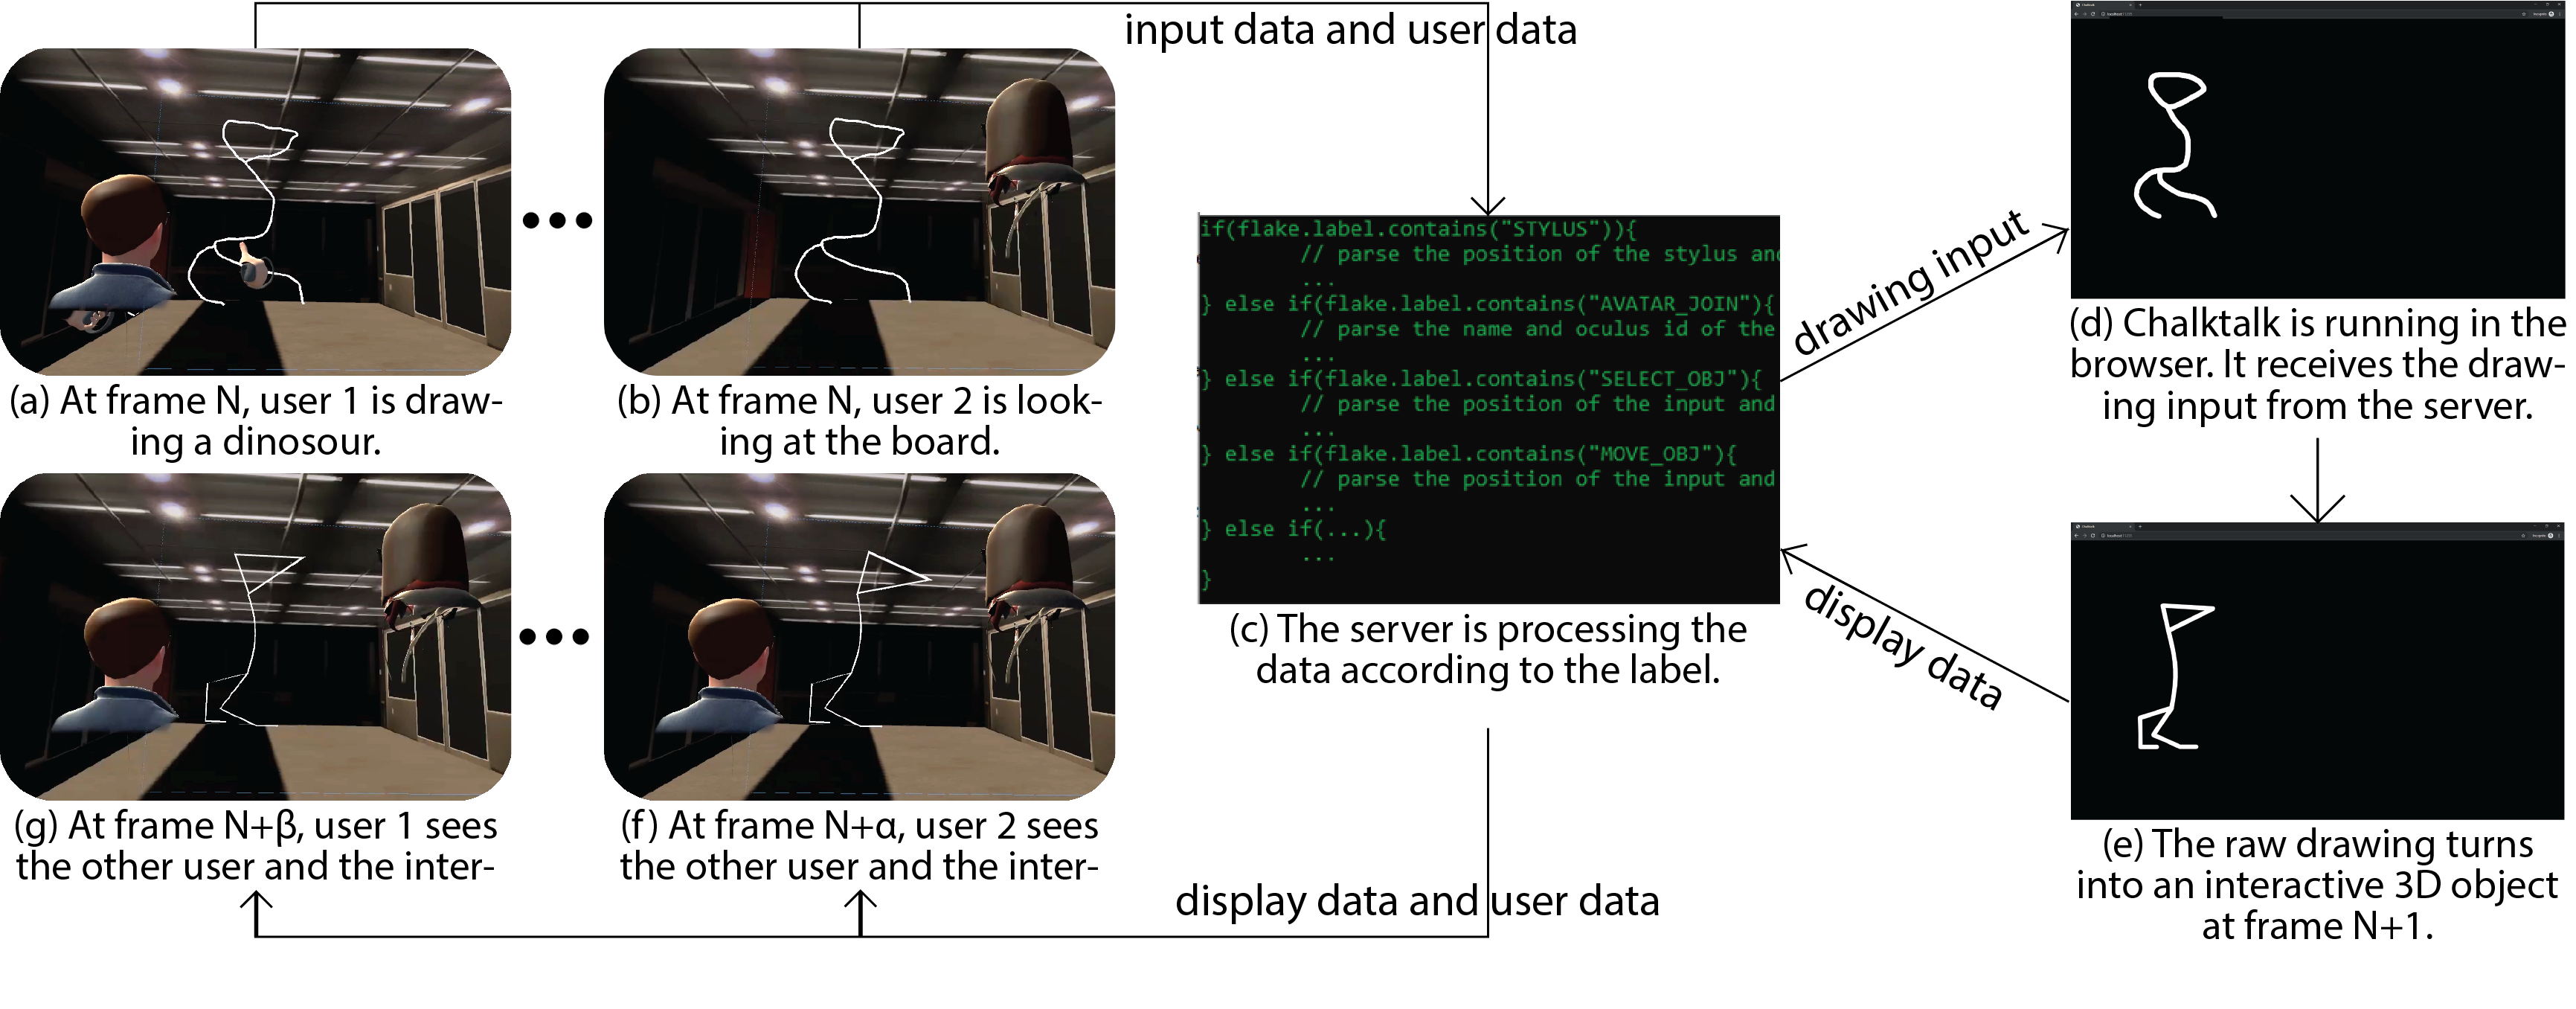
\includegraphics[height = 6.5cm]{Figure2.png}
 \caption{The workflow of CollaboVR. Figure (a) and (b) illustrate the third-person perspective view of the VR clients before data synchronization. Then, the input data and the user data, such as avatar data and audio data, are wrapped with a unique label and transmitted to the server. Later, the server processes the data based on the label in figure (c). The input data goes to Chalktalk, and the user data is broadcasted to all the clients. Chalktalk processes the input data. For example, the raw drawing from user 1 turns into an interactive dinosaur, as shown in figures (d) and (e). All the display data is broadcast to all clients through the server. Finally, users 1 and user 2 can see the 3D object and each other as shown in figure (f) and (g). In addition, the dinosaur is actually an interactive software object having well defined behavior. Here we can see it in two different poses.}
 ~\label{fig:workflow}
\end{figure*}

CollaboVR consists of a star network. The network is written in Node.js and C\# and it synchronizes data across devices and supports custom data formats. For CollaboVR, we have two kinds of information: rendering data and user data. For rendering data, we first pass the user input from each client to the server. Then, the server transmits the user input together with its user identifier to the application. Next, the server receives the serialized display data from the application. Finally, the server broadcasts the display data to each client for rendering. For user data, we directly broadcast the user avatar and audio data to each client after it has been received.

CollaboVR consists of rich interactions for manipulation of drawings. After the clients receive and render the display data from the application, the display data are considered as interactive objects in a 3D world. We provide manipulation of these objects for users to easily express their ideas. This manipulation includes duplication, linear transformation (rotating, scaling and translation), deletion, and colorization.

Deploying CollaboVR requires only a VR device running Unity for each client, a server machine running Node.js and an optional router for ensuring low latency for data transmission. If a VR client needs to run on a Windows machine, the server code could run on one of the client machines. If a router is not available for setup, the server and all the clients can communicate via their external IP addresses.

% talking about architecture with figures
% Explain the entire pipeline and Chalktalk

Figure ~\ref{fig:workflow} presents the per-frame workflow of CollaboVR. First, figure~\ref{fig:workflow}(a) and figure~\ref{fig:workflow}(b) illustrate the third-person perspective view of the VR client before data synchronization. The user in figure~\ref{fig:workflow}(a) is drawing a dinosaur to present his or her favorite animal. The user in figure~\ref{fig:workflow}(b) is waiting. Then, the data, including both users' identifiers, avatar information, audio and the drawing input information is serialized and sent to the server. As figure~\ref{fig:workflow}(c) illustrates, different data are processed with different labels such as \verb|AVATAR_JOIN|, \verb|STYLUS|, \verb|SELECT_OBJ|, \verb|MOVE_OBJ|. The server behaves as a stateless machine. The server sends the drawing input related data to the application API and broadcasts user data to all clients. The application then receives the drawing input data from the server as shown in figure~\ref{fig:workflow}(d). The application (Chalktalk) processes the input and turns the drawing into 3D objects, as shown in figure~\ref{fig:workflow}(e). We can see that the freehand drawn dinosaur becomes a 3D dinosaur capable of interactive animation. Our protocol serializes \verb|DisplayData| from the application (Chalktalk) and sends that data to the server. The server broadcasts \verb|DisplayData| to all the clients. Finally, all the VR clients can see the interactive 3D objects and each other, as shown in figure~\ref{fig:workflow}(f) and figure~\ref{fig:workflow}(g).

\section{Design Space}
We propose two variables in the design space of CollaboVR: user arrangement and input orientation. Building on previous work on workspace awareness, we focus on maintaining and enhancing workspace awareness, to enable participants to work together more effectively. We added a control variable that users can use to alter their views of other participants. In other words, they can manipulate the spatial arrangement by which they see other users. 

Inspired by previous work on collaborative sensemaking, we notice that multiple and shared large displays are useful for collaborative work in terms of 2D information. CollaboVR is an immersive 3D graphics world. Instead of "display", we pre-placed multiple "interactive boards" in the virtual environment, meaning that if the z coordinate of the content is 0, the content will be placed on the interactive board. If the content has a positive or negative z coordinate, users will see that the content floats in front of or behind the interactive board. By default, the interactive board is placed vertically like a blackboard. We allow users to rotate the vertical tilt of the interactive input board from 0$^{\circ}$ to 90$^{\circ}$. In order to reduce the learning curve for users, we simply provide two options: vertical (0$^{\circ}$) and horizontal (90$^{\circ}$).

\begin{figure}[t!]
 \centering
 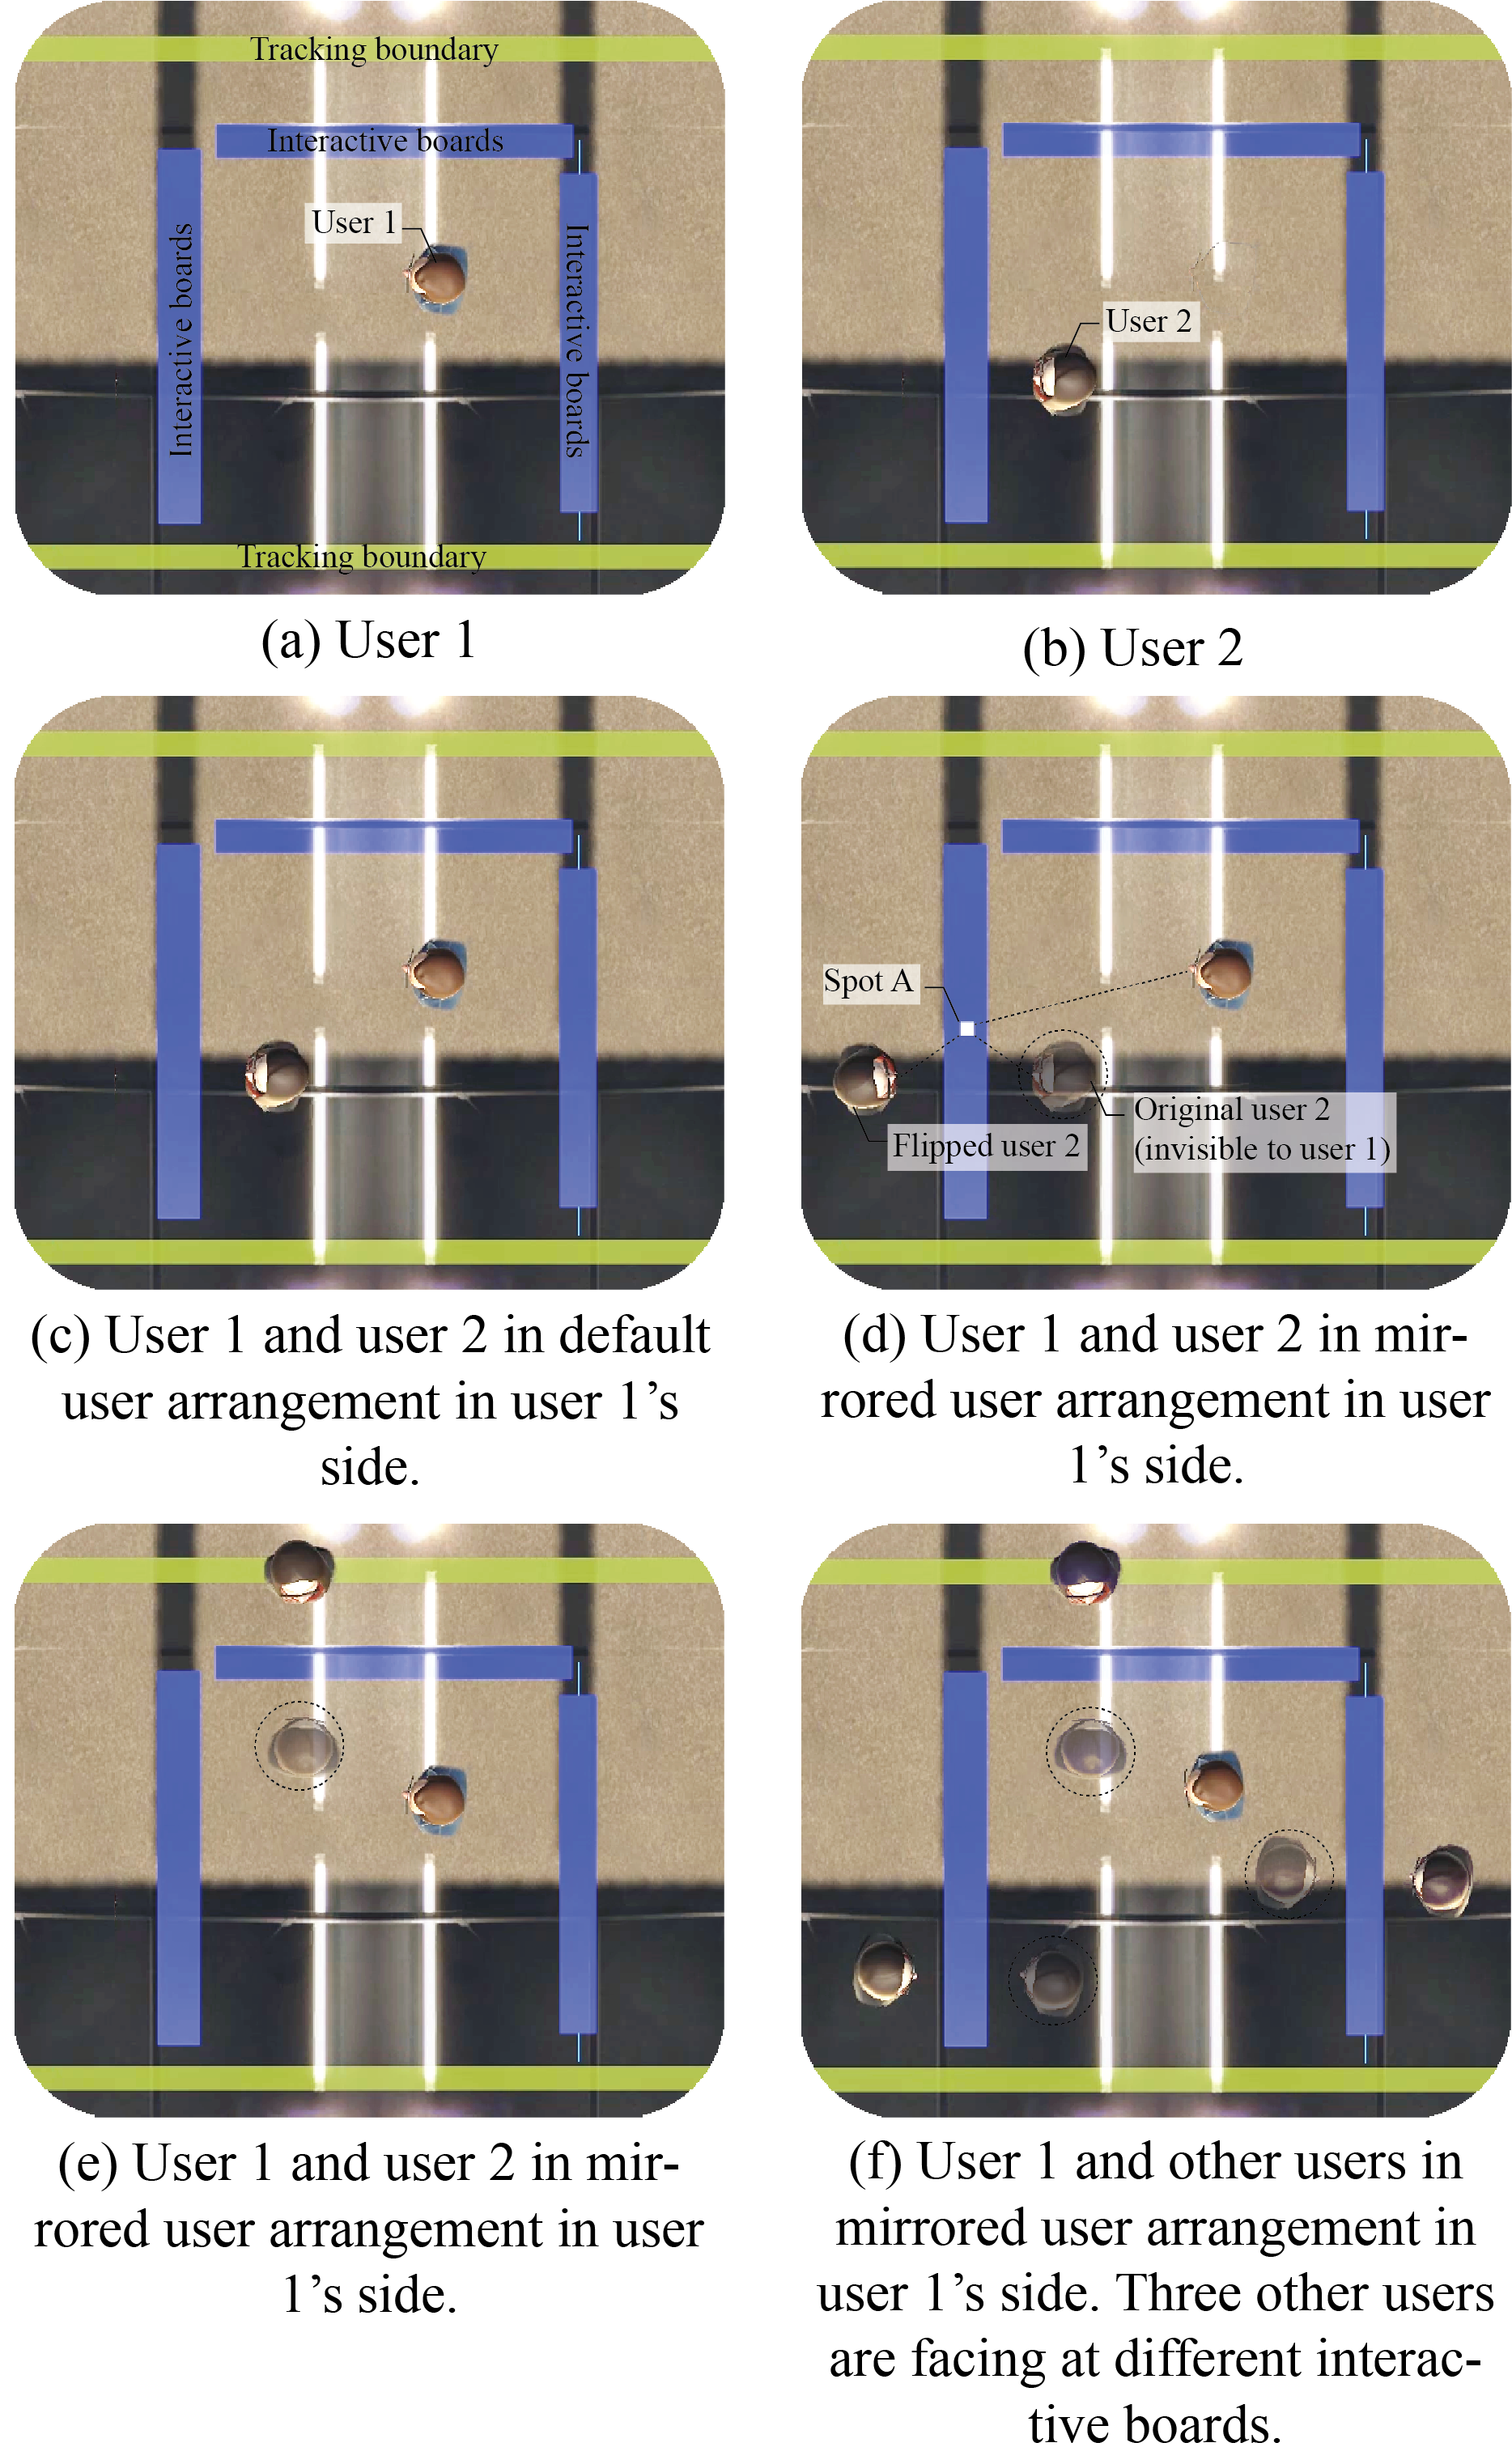
\includegraphics[width=0.95\columnwidth]{Figure3.png}
 \caption{Design space: user arrangement. From figure (a) to (f), blue rectangles represents interactive boards, and green rectangles represents the boundary of the tracking area. All sub-figures are captured as top-down view. Figure(a) and (b) illustrate the original locations of two users. Figure(c) demonstrates the default user arrangement. Figure (d) demonstrates mirrored user arrangement. The transparent avatar inside the dashed circle shows the original user 2. In mirrored user arrangement, it is flipped to the other side of the interactive board, so this transparent avatar is invisible in user 1's side, while what user 1 sees is the "flipped user 2". Assuming "spot A" is the area which two users are looking together. The gaze interaction is maintained after flipped. Figure(e) illustrates the scenario when user 1 and user 2 are looking at different interactive boards. User 1 can barely see user 2. Figure (f) presents the case that three other users are looking at different boards.
 }~\label{fig:userarrangement}
\end{figure}

\subsection{User Arrangement}
We provide two user arrangements for CollaboVR: (1) default and (2) mirrored. A default user arrangement means that the virtual environment of each user will be overlapped directly. As figure~\ref{fig:userarrangement} demonstrates, the green rectangle roughly shows the available tracking area. The blue rectangles show the interactive boards. All the sub-figures are top-down views. Figure~\ref{fig:userarrangement}(a) and (b) illustrate the original position of two clients in their own sides. Figure~\ref{fig:userarrangement}(c) shows the default user arrangement. The clients see the other participants in their original positions. For mirrored user arrangement, all the other users' locations are flipped to the other side of the interactive board. In figure~\ref{fig:userarrangement}(d), user 1 is in a mirrored user arrangement, so user 2 is flipped to the other side of the left interactive board because user 2 is looking at that board. Now let's take a look at the gaze interaction. Spot A is the same content that both users are looking at. After the flipping operation, the gaze direction of user 1 and user 2 are maintained. Different from FacingBoard~\cite{li2014interactive}, the content is not mirror reversed so the content is still correct to the viewer. In this user arrangement, the users can see each other for better workspace awareness. Figure~\ref{fig:userarrangement}(e) illustrates the scenario that two users are looking at different interactive boards. User 2 doesn't block the view of user 1, and they can barely see each other when their focused boards are different. Figure~\ref{fig:userarrangement}(f) illustrates how we process multiple users in this setup. Each user will be flipped based on their looking direction.

\subsection{Input Orientation}
CollaboVR enables the user to adjust the interactive board for input to be either vertical or horizontal. By default, the interactive board is vertical as a large display, but in 3D. As figure~\ref{fig:teaser}(a) demonstrates, the user's experience is close to writing on a white-board. When user turns on the horizontal interactive board, it is close to writing on a tablet or desk, as seen in figure~\ref{fig:inputorientation}. For other users who are not writing, the content is rendered in real time on the vertical board, see figure~\ref{fig:inputorientation}(a). By doing this, we avoid the situation that the content is not readable for all the users around a table in real life. When user is writing on the horizontal board, he or she is free to look at the personal horizontal board or the shared vertical board. (See the dash dot representing potential gaze directions in figure~\ref{fig:inputorientation}(b).) Moreover, the content on the horizontal board is different from the content on the shared vertical board in two points. One is the scale. Considering that the reach distance when writing on a horizontal plane is smaller than on a vertical plane, we adjust the scale of the horizontal board. The other is the dimension. We squeeze the content on the horizontal board. (See how the table looks in figure~\ref{fig:inputorientation}(b).) We implement squeezing because we want to simulate a tablet-style input, and keep the designing space clean as well. To enhance the awareness of where the user is writing, we render the projection point of user's controller as a 3D/2D cursor. (See the torus in figure~\ref{fig:inputorientation}.)

\begin{figure}[tb!]
 \centering
 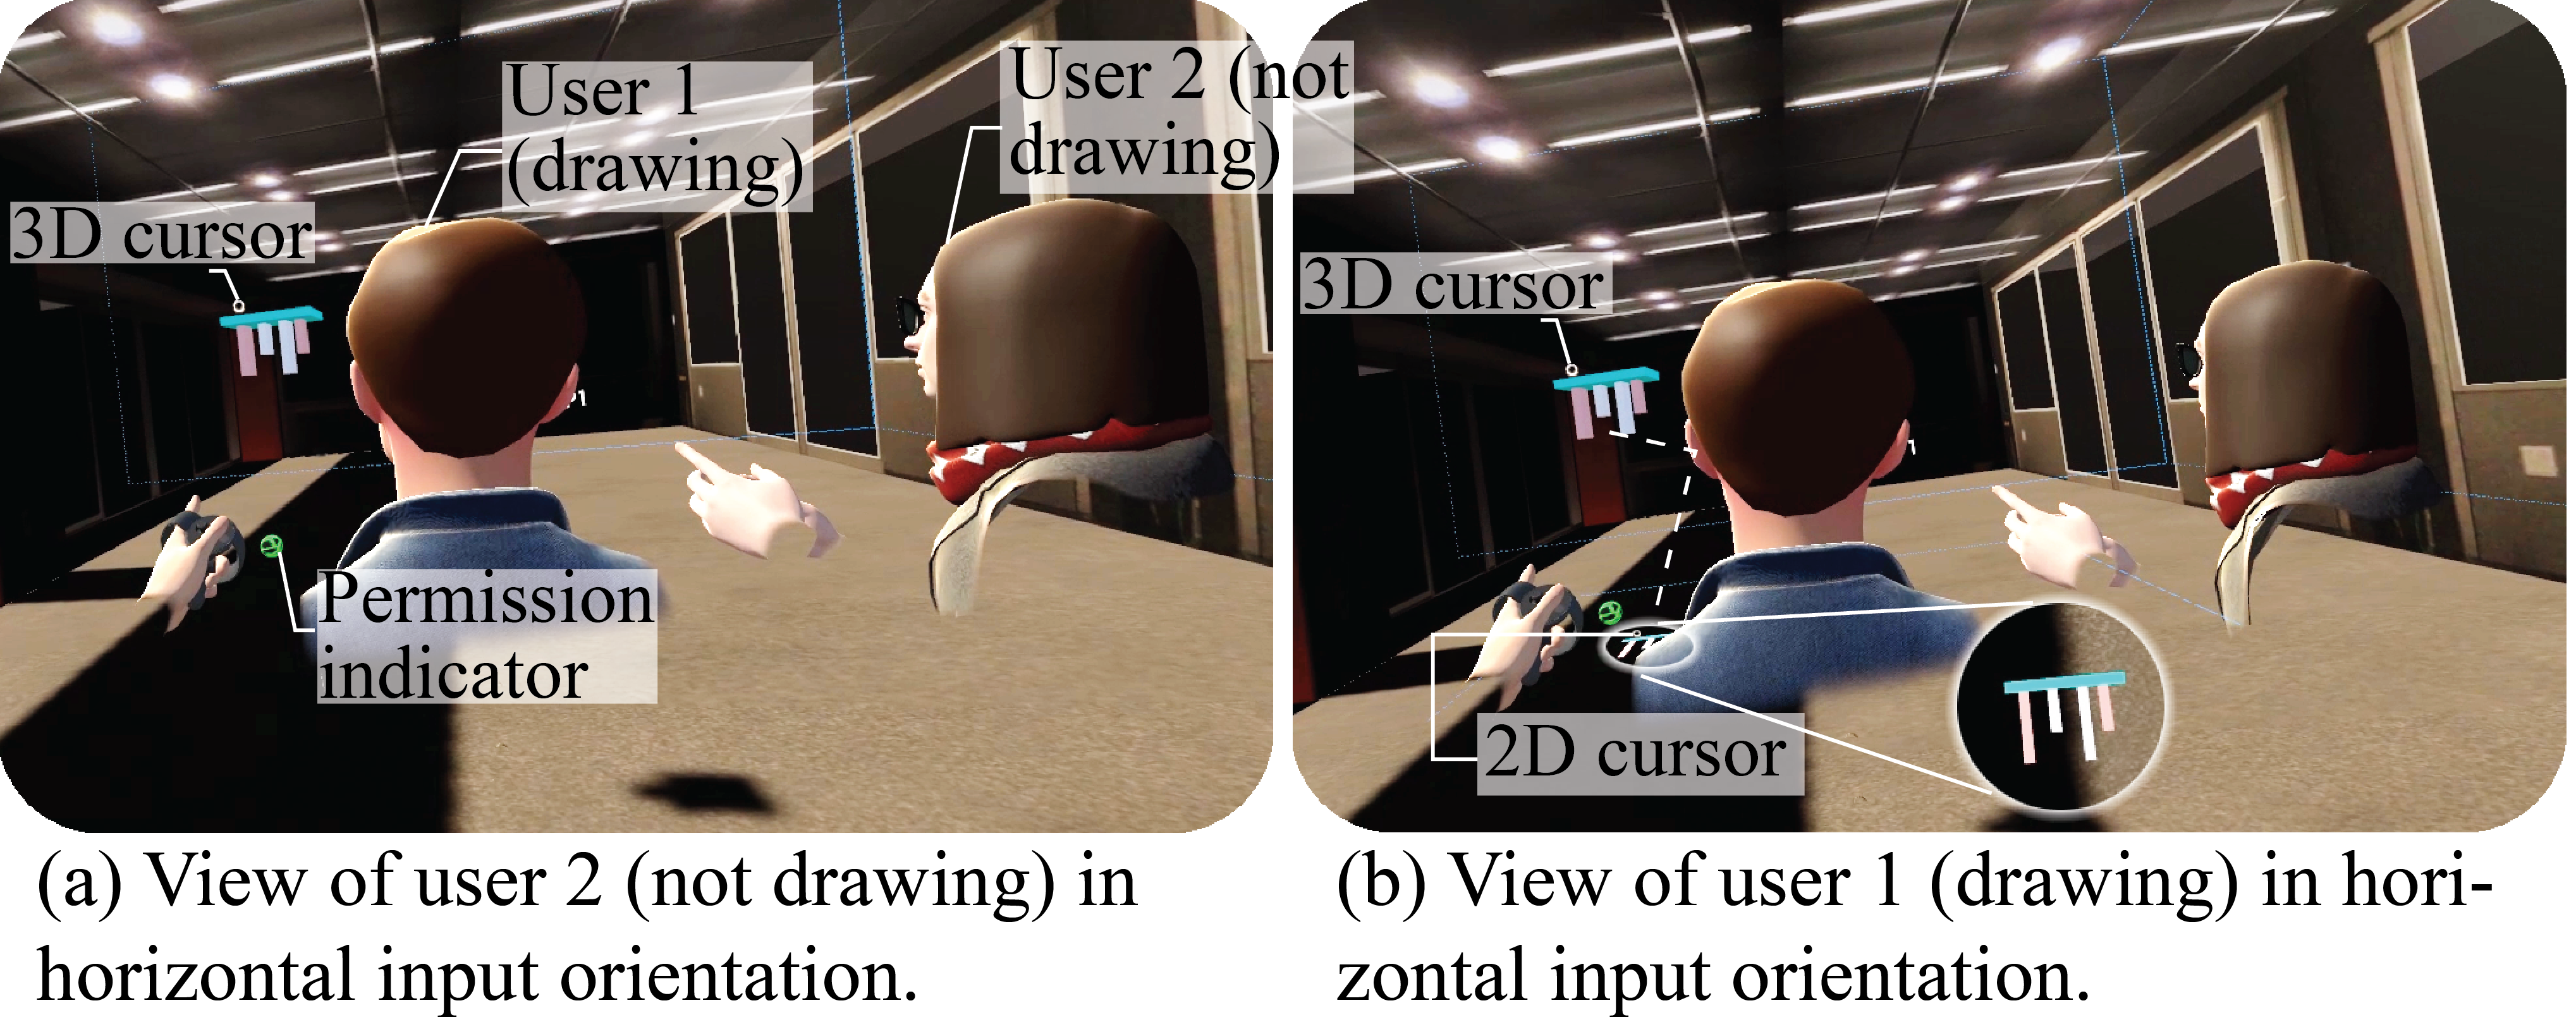
\includegraphics[width=0.95\columnwidth]{Figure4.png}
 \caption{Design space: input orientation. Figure(a) demonstrates the view from user 2, who is not drawing. To user 2, horizontal input orientation has no difference from default input orientation. Figure(b) demonstrates the view from user 1, who is drawing. User 1 can see the drawing in 3D from the vertical board and in 2D from the horizontal board at the same time.
 }~\label{fig:inputorientation}
\end{figure}

\section{System Implementation}
To build CollaboVR, we implement a network framework with a flexible protocol, a calibration approach for co-located users, user interface for drawing manipulation and other functions.

\subsection{Network and Protocol}
The network is a star network using UDP. We chose UDP because we value low-latency. The user data and rendering data need to be transmitted every frame. The server-side code is written in Node.js and the client code is written in Node.js and Unity C\#. We defined a \textit{synchronizable object} as an object that needs to be synchronized each frame for the client who registered it. Each synchronizable object has a label and data stream. The label is a unique identifier for the client to register. The data stream includes the frequency of sending this object and the real-time data. We provide two types of frequency in the system: one-time and per frame. A one-time synchronizable object is actually a command. It does not happen for each frame and does not need to be synchronized for each frame. For the command object, we use two-way handshaking. The client sends the object to the server, the server returns an object including acknowledgement back to the client, then the client deregisters the object with this local label. The per frame synchronizable object could be the current avatar representation, the audio data or the display data from the application. We design a protocol to wrap all the display data. The data protocol includes information of all the rendered lines and meshes by encoding their attributes, such as the width of the lines and shape of the meshes. Each client deserializes the data from the server and renders the points as lines and meshes.


\begin{figure}[tb!]
 \centering
 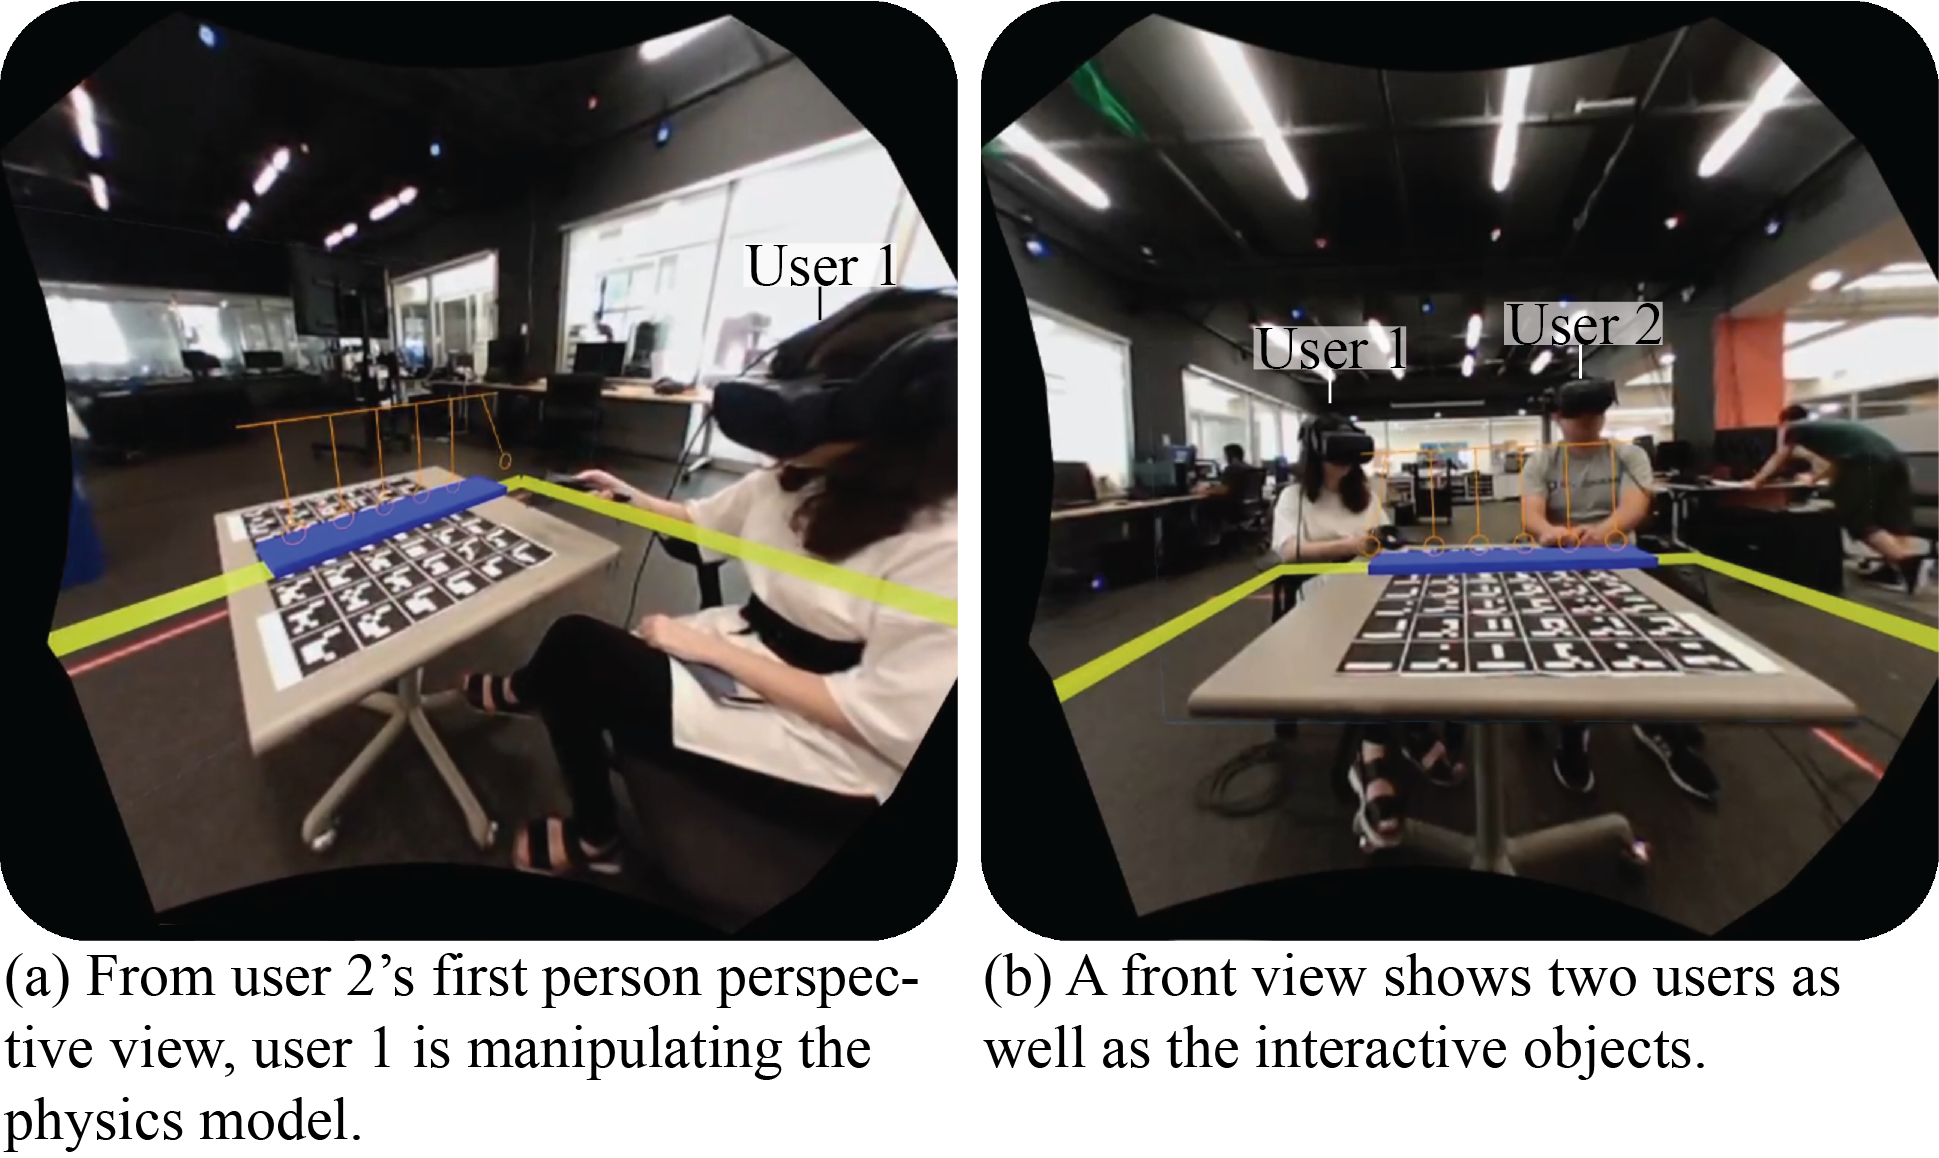
\includegraphics[width=0.95\columnwidth]{Figure5.png}
 \caption{Co-located user setup with HTC Vive Pro. Figure (a) is the first-person perspective view from user 2. User 2 sees that user 1 is presenting a physics model. Figure (b) is the front view including both users.
 }~\label{fig:vivepro}
\end{figure}

\subsection{Calibration for Co-located Scenarios}
CollaboVR works for both co-located and distributed scenarois. For distributed users, we simply overlap their virtual environments because they do not have any spatial relationship in reality. For co-located users, we need to calibrate all the users, so they are all in the same coordinate system. The key idea for calibration is that different clients should have a shared proxy. For example, a shared image is provided to all the co-located users in that environment. Vuforia~\cite{Vuforia} is widely used for image recognition and tracking. Similarly, a shared map is helpful too~\cite{Hololens}. Here we use HTC Vive Pro as the co-located device. Technically, HTC Vive Pro is capable of both VR and MR. We only use VR mode in our system. Meanwhile, MR mode helps us explain the co-located user setup as figure~\ref{fig:vivepro} illustrates. The shared proxy in Vive system is the Vive base station. Each machine running Vive can retrieve the transformation information of the base station. Because all machines (assuming $N$ machines) have their own coordinate systems, we have $N$ pairs of position and rotation of base station in different coordinate systems. We chose one base station as the proxy based on the unique serial number. Then, we used the first client that connected to the server as the reference node. Later, all the following clients applied the inverse matrix between the base station of reference node and their own base station to their VR environments. In figure~\ref{fig:vivepro}, user 1 is drawing a physics model. Figure~\ref{fig:vivepro}(a) presents the first-player perspective view from user 2, and figure~\ref{fig:vivepro}(b) presents a front view of the scene.

\subsection{Drawing Manipulation}
CollaboVR includes a user interface for users to manipulate the objects after drawing. We provide the functionality of duplication, transforming, deletion and colorization. To achieve this, we designed a pie menu triggered by the controller. The following is the workflow for a user's manipulation: first, place the controller so that it hovers over the drawing of interest; second, press the thumbstick of the dominant controller; and then, the pie menu appears as figure~\ref{fig:userinterface}(c); later, move the thumbstick to select the specific menu (see figure~\ref{fig:userinterface}(d)); afterward, apply corresponding movement in terms of the command and release the thumbstick. If the menu is deletion, the operation executes immediately after release. If the menu is transformation, the user must move the controller one more time to complete rotation, scaling or translation. If the menu is copy, the duplicated object will be placed at the position where the user releases the thumbstick (see figure~\ref{fig:userinterface}(a)). The color palette is toggled by button one, illustrated in figure~\ref{fig:userinterface}(a). The user can drag the color from the color palette to any drawing like world builder~\cite{worldbuilder}.

\begin{figure}[b!]
 \centering
 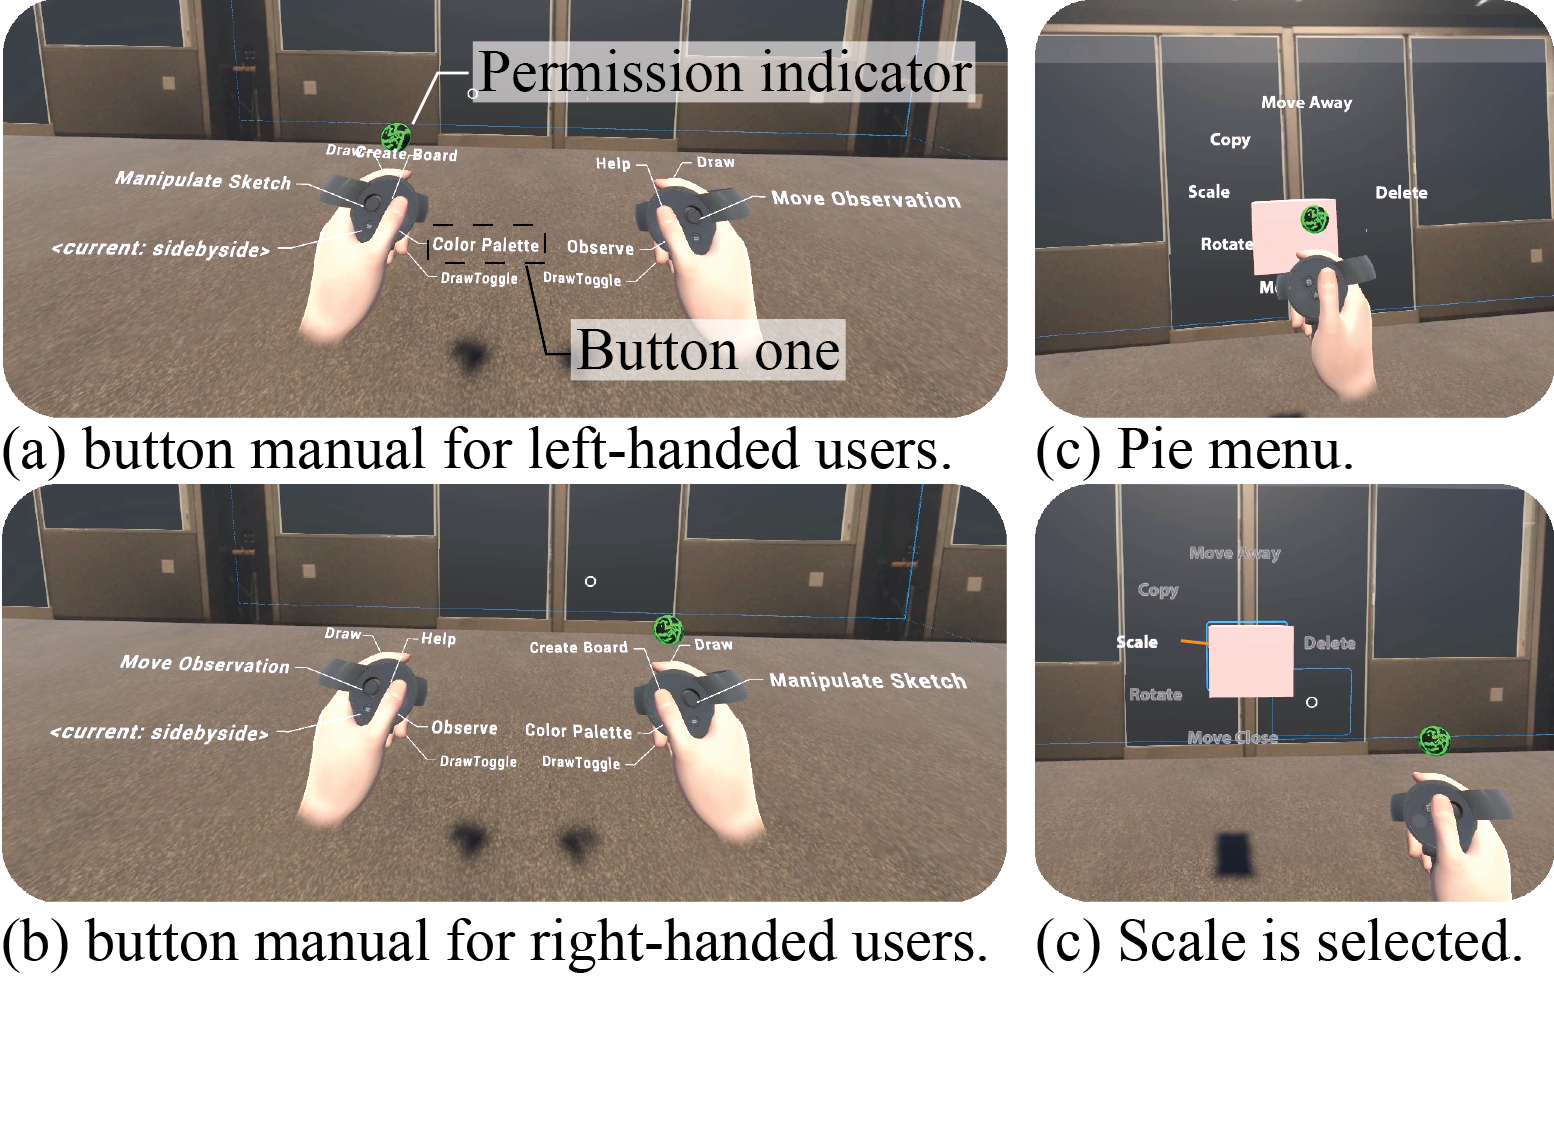
\includegraphics[width=0.95\columnwidth]{Figure6.png}
 \caption{User interface for drawing manipulation. Figure (a) and (b) present the button manual for left-handed and right-handed user. The permission indicator represents which hand is dominate hand, as well as the 3D cursor. Figure (c) illustrates the pie menu triggered by thumbstick (see "Manipulate Sketch" in figure (a)). Figure (d) illustrates the behavior when one menu is selected. for example, scale.
 }~\label{fig:userinterface}
\end{figure}

\subsection{Other}
The controller's trigger switches the commands of the two controllers (see figure~\ref{fig:userinterface}). As the user's view might be blocked by other users' avatar, we implement a spectator mode. Users can see the view from different users in the lower right corner. To encourage all users to work on the task together, we implement a permission strategy. Only one user we can draw at one time. Once the user who is drawing releases the permission, other users can grab permission to draw. Figure~\ref{fig:userinterface} shows the permission indicator.

\section{Use Cases}
CollaboVR is designed as a reconfigurable framework for users to communicate in VR. Here, we envision the potential user cases for CollaboVR.

\subsubsection{Daily Life Schedule and Brainstorming}
CollaboVR can be used for daily life scheduling as shown in figure~\ref{fig:teaser}(a). With the default user arrangement and input orientation, the experience is close to whiteboard writing. CollaboVR enables freehand drawing, so users can write and draw their plans and coordinate with friends. Shapes and colors are useful while scheduling. When they have different ideas, users can easily duplicate the current drawing onto another interactive board to express new alternatives.

\subsubsection{Presentation}
CollaboVR can be used for presentation as shown in figure~\ref{fig:teaser}(b). By enabling the mirrored user arrangement and the default input orientation, the presenter and the audience will be placed on different sides of the content. It is easy for the presenter to know where the audience's focus is, and it is useful for the audience to follow the presenter's gesture and content at the same time.

\subsubsection{Spatial Arrangement}
CollaboVR can help with spatial arrangements, especially for 3D scenarios. Imagine that the user has just moved in to a new apartment and needs to discuss the placement of the furniture with a roommate. As figure~\ref{fig:teaser}(c) demonstrates, the user can draw furniture with a combination of primitive shapes and place them directly at the preferred locations. Spatial arrangement is difficult to describe clearly through words and gestures, and it often requires multiple views when using drawings. CollaboVR can be helpful for such scenarios.

\subsubsection{Item Design}
CollaboVR can help with collaborative design. By enabling the mirrored user arrangement and horizontal input orientation, users can draw their items in detail with friends. The experience is close to drawing on a digital tablet with a pen. Other users can explain their opinions while pointing at the area of interest.

\section{User Study: System Evaluation}

In this study, we evaluated the interaction cycle, design variables and prototype implementation of CollaboVR. We were interested in how participants interact with the system. During the study, we collected primarily qualitative feedback to gain insight into the experience of using the system.

\subsection{Tasks and Procedure}
\subsubsection{Introduction and Training}
Participants were grouped by four. Each group was first introduced to the user study and gave consent for video recording. Then they were given a 10-minute lecture through a large monitor on the concept of Chalktalk. During the lecture we demonstrated how to do freehand drawing and how to create pre-defined 3D objects.
In the next 10 minutes, participants were given a live demo on how to use CollaboVR. As part of the demo, an experimenter put on the headset and described how to use each button on the controller as well as the functionality of the system, including obtaining permission to draw, manipulating drawings and objects in 3D, and other functionalities.
After that, each participant was moved to a different location. They learned how to interact with CollaboVR individually until all of them were able to conduct drawing and manipulation (this took around 10 minutes). Finally, they were brought to the shared virtual environment for design tasks. 

\subsubsection{Living room design}
Next, all of the groups were asked to experience three 10-minute sessions. 
Each session featured different combinations for user arrangement and input orientation: condition 1(C1) is default user arrangement and input orientation; condition 2(C2) is mirrored user arrangement and default input orientation; condition 3(C3) is default user arrangement and horizontal input orientation.
We counterbalanced the order of the conditions for each group using Latin Square. In each session, the participants were asked to design a living room  containing only three items: a table, a chair and a couch. 
Each participant picked one item and wrote down their designs for the items and their layout of the three items. They then used CollaboVR to express their original ideas and reach an agreement for the living room design. After each session, they wrote down their final decisions for the design of the living room. (The writing was collected for further analysis.)
We provided three items for the group (of four people), so they needed to resolve conflicts and come to a consensus about the design of a living room through our system.

\subsubsection{Semi-structured interview}
Upon completion of all the sessions, we presented the participants with a set of statements and asked them to rate how much they agreed with each of those statements on a 7-point Likert scale. We then administered a semi-structured interview asking about their experience, trying to gain insight into usability and use cases of the system.

\subsection{Participants}
We recruited a total of 12 participants (5 females and 1 left-handed; age range: 20 - 30, $M=23.58$, $SD=3.45$) via campus email lists and word-of-mouth. None of the participants had been involved with this project before. The participants have various VR experience (Rating scale, 1 (less experience) to 7 (more experience), $M=4.08$, $SD=1.83$).

\subsection{Apparatus}
CollaboVR was implemented in Unity on Windows desktops with Nvidia GTX 1080 cards. We used Oculus Rift CV1 with two Oculus Touch controllers for the study. Before the experiments, we paired the controllers with the headset on four computers. We connected the four computers to the router through Ethernet cables.

\subsection{Data Collection and Analysis}
Through the survey and interview, the study mainly focused on the system usability evaluation and qualitative feedback. Besides, we conducted one-way analysis of variance (ANOVA) statistical tests to examine the variance between different user arrangement and input orientation on task performance, which is defined as the details of the living room design for each session per group. We analyzed what they wrote before and after each session by calculating the quantity of the details, such as color, shape, texture and layout. Our null hypothesis is that across different user arrangements and input orientations, there is no difference in task performance. We predict that (1) the mirrored user arrangement would foster higher performance and (2) the horizontal input orientation would lead to lower performance. Questionnaire data that related to usability of user arrangement and input orientation were analyzed using repeated measures analysis of variance (RM-ANOVA). The level of significance was set at $p<0.05$.

\subsection{Results and Discussion} 
\begin{figure}[tb!]
 \centering
 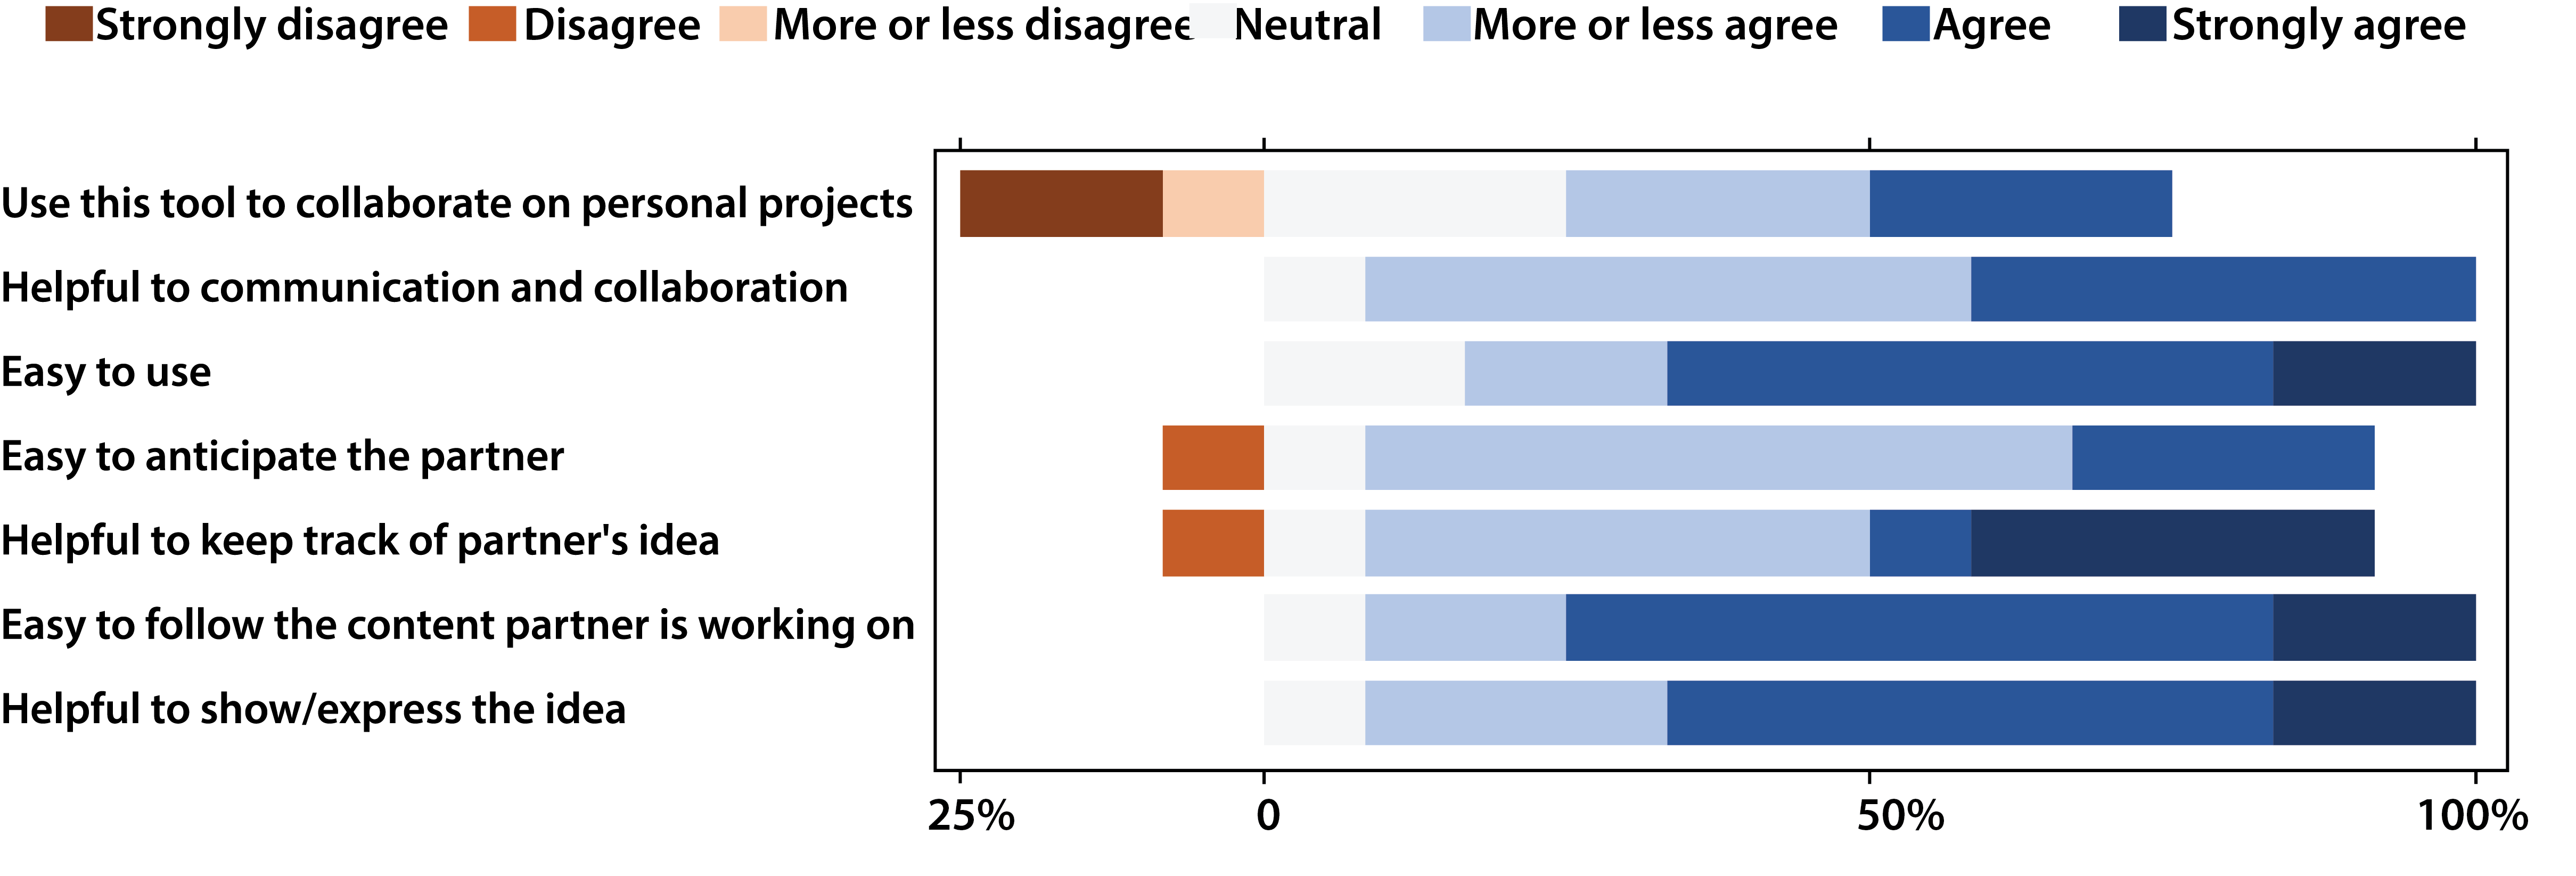
\includegraphics[width=0.98\columnwidth]{usability.png}
 \caption{Agreement distribution of the post-task questionnaire for system usability. The further bars extend to the right, the more users agree.
 }~\label{fig:usability}
\end{figure}
\subsubsection{Usability}

\begin{table*}
  \centering
  \begin{tabular}{l C{2.2cm} C{2.25cm} C{2.15cm} C{2.8cm} C{2.8cm} }
    % \toprule
    & Condition 1 (C1) & Condition 2 (C2) & Condition 3 (C3) & ANOVA between C1 and C2 & ANOVA between C1 and C3 \\
    \midrule
    Performance & 9.67 & 9 & 5.33 & $F_{(1,5)} = 0.21$ & $F_{(1,5)} =8.45$ \\
     & (1.53) & (2) & (2.08) & $p = 0.67$ & $p = 0.04*$\\
    Easy to use & 5.67 & 6 & 4 & $F_{(1,23)}=0.65$  & $F_{(1,23)}=8.59$\\
     & (0.98) & (1.04) & (1.71) & $p=0.43$ & $p=0.008*$\\
    % \bottomrule
  \end{tabular}
  \caption{Mean values and standard deviations (in parentheses) for performance and questionnaire results, and ANOVA results between condition1 and other conditions.}~\label{tab:result}
\end{table*}

CollaboVR's pipeline was quickly understood by all users. Knowing how to get permission, conducting freehand drawing, drawing 3D objects, manipulating the drawing afterwards, and spectating other users. 83.33\% of the participants agreed that the system is easy to use ($M=5.67$, $SD=0.98$). \textit{``It is intuitive to do the drawing in 3D.''}. Participants found out the permission strategy design is useful: \textit{``having to get permission to draw is really good at making the environment easier to work in.''}(P7,F).
91.67\% of the participants agree that it is helpful to show/express the idea ($M=5.75$, $SD=0.87$). 
\begin{quote}
    There could be merit once you're doing something more complex to 'hey look, this thing, let's do x,y,z...' and that's a lot easier to use this system.(P11,M)    
\end{quote}
Furthermore, 91.67\% of the participants agreed that it is easy to follow the content partner is working on ($M=4.92$, $SD=1.08$), and 83.33\% of the participants agreed that it is helpful to keep track of partner's idea ($M=5.42$, $SD=1.50$). Partly because the users can \textit{``move themselves easily''}(P1,M), they can easily follow the partner's drawing and thoughts.
In fact, 75\% of the participants agree to use this tool to collaborate on personal projects ($M=4.17$, $SD=1.75$). 
\begin{quote}
    That's what I'd use for my own work. It's like a more --not quite as artsy -- business tool. I would use it to get my ideas across to people(P8,M).
\end{quote}
Similarly, P11(M) thought, \textit{``it's totally a great prototyping idea/prototyping system. Can't say it'll replace AutoCAD, but in a few years it will do that.''}.

In addition, 91.67\% of the participants thought CollaboVR is helpful to communication and collaboration ($M=5.33$, $SD=0.65$), and 83.33\% of the participants agreed that they can anticipate what the partner would do next ($M=4.92$, $SD=1.08$). P3(F) commented that, \textit{``when [another user] started to draw the legs for the table, I quickly get his idea about the design of the legs, so he doesn't need to say what kind of legs he wants.''}. The participants found it an engaged experience and love to spend more time with friends. \textit{``It's definitely a fun environment, entertaining.''}(P7,M).

\subsubsection{User Arrangement}
Based on table~\ref{tab:result}, there are no significant differences between the default user arrangement and mirrored user arrangement for task performance and ease of use. However, 58.33\% of the participants rated this session as the favorite one, probably because the users have better workspace awareness in this session and because they can keep the content and the others in view together. Quotes, \textit{``[...] mirrored, it is easy and convenient to communicate with others.''} from P3(F) and \textit{``people didn't block my view, and I could see the content clearly.''} from P5(M) shared the similar thoughts. 33\% of the participants preferred the default setup most. P2(M) commented, \textit{``because it is comparable to reality.''}. P1(M) had similar opinion. We thought there might be two reasons. One is that some participants have less VR experience. This session is the closest setup comparing to real life, so they can get used to it quickly. The other reason was that the mirrored user arrangement will flip other users to the other side of the interactive board which might lead to the feeling of \textit{``i felt really far away from everyone.''}(P7,F).

Next, we collected feedback of the ideal scenarios for different user arrangement. Mirrored user arrangement could be user for delivering a presentation. P4(M) suggested that because \textit{``you can better control your drawing meanwhile keep an eye on people's reaction through the mirror.''}. P5(M) thought about it from a student's view, \textit{``kind of felt like Khan Academy in 3D vision.''}. This is quite consistent with previous work focusing on face-to-face experience. P9(F) thought she can benefit from this setup when brainstorming because no one is blocking the view, \textit{``uou can see everybody but you have your own space.''}.

\subsubsection{Input Orientation}
From table~\ref{tab:result}, we can see that significant differences were found between different input orientation. Horizontal input orientation negatively impacts performance and usability. P8(M) commented that \textit{``I think this setup could be really good.''}, \textit{``like the tablet.''}, and \textit{``the horizontal board should be slanted more.''}. P8(M) is a 3D modeler who frequently used tablet a lot for detailed drawing, so he has more experience with the input in tablet style. However, P12(F) felt \textit{``that type of idea works well with a physical tablet''}. One reason why this setup has negative impact is probably that most participants are not familiar with such an input. We rendered the same thing on both the personal horizontal board and the shared vertical board. Some users found it difficult to create the correct mapping between the two views. On the other hand, users drawing horizontally can rest their elbows on the chair arm when drawing, so they enjoyed drawing longer than when drawing in mid-air. Furthermore, the participants tended to draw richer details because they felt liking holding a pen. 8.3\% of the participants prefer this setup the most and emphasized that \textit{``I had more control over what I was drawing.''}. In summary, horizontal input orientation enables users to draw or write like on a tablet, which encourages the users to draw for a longer time and brings more control to the users. However, users may need more time to get used to it.

When discussing the suitable scenarios for this setup, P8(M) thought a live demo or presentation could be beneficial from this, especially for a time-consuming one. He described \textit{``himself giving a presentation to other people looking at the big monitor while an audience was looking at the large monitor-like board.''} and \textit{``just want to focus on the board.''}. Meanwhile, P11(M) thought it would be helpful for collaborative design and suggested us to replace the controller with a pen. We found all of the thoughts inspiring.

\section{Discussion, Limitations and Future Work}
The results of our study roughly proved that CollaboVR can be used to communicate with others for non-expert use, such as brainstorming and presentation. The system is relatively easy to use and the experience is engaging and entertaining. Participants are willing to hangout with friend in the system. Considering two key variables we proposed, mirrored user arrangement has positive but not significant effects on the experiment. Participants felt that others are synced up with them because of greater awareness. Horizontal input orientation indicates the potential for detailed and longer time experiences. However, its learning curve is larger than other setups for users who have less tablet experience. In addition, a physical tablet~\cite{sensel} or a pen~\cite{wu2017dodecapen} as input could be helpful for this setup. 

One limitation of the user study is the lack of diversity of the participants. Most participants are from the department of computer science, and the age range is not wide enough. The results of our study may therefore not be easily generalizable to other users, such as artists, financial people and older adults. Another limitation of the system is that participants found it difficult to track who was speaking. Either visual hints like attaching a speaker icon to the avatar or mouth tracking would be useful.

In the future, we plan to conduct more user studies to explore how CollaboVR affects the communication in different scenarios, such as presentation and brainstorming. Inspired by P7(F), supporting search engine is an interesting direction. We also want to investigate other user arrangements and input orientations.

\section{Conclusion}
In this paper we presented CollaboVR, an open-source reconfigurable framework for distributed and co-located multi-user communication in VR. We described the system architecture, the design of two key variables (user arrangement and input orientation), the rich user interface, and its implementation. The system was evaluated in a user study showing that participants can easily interact with the system, and found it entertaining and useful for communication. We discovered that participants stated they would consider CollaboVR as a daily-life tool and can envision its potential. We also evaluated the key variables in terms of both usability and performance. Users reported that different combinations of two key variables work differently for different collaborative purposes, such as brainstorming, presentation, and design.

\section{Acknowledgments}
We thank all the volunteers for participating in our experiments and video shoots.

%In daily life while speaking to others, we commonly use gestures or visual aids~\cite{tversky2003human} to help present ideas, either subconsciously or purposefully. Visual aids can be drawn on paper, a whiteboard\cite{cherubini2007let}, or a screen via desktop sharing in video conferences. A key task for collaborators is visually, physically, and cognitively following the content being drawn and the people who are speaking with. They need a clear view of the content under discussion and need to be aware of other collaborators' presence when communicating~\cite{ishii1992clearboard}. They should also understand and be able to reason about what is being shown and said. 
%According to Regenbrecht et al.~\cite{regenbrecht2015mutual}, facial interaction like eye contact and mutual gaze has always been recognized as an important requirement for effective visual communications. That suggests it is helpful during communication to look at the person who is talking or at least be aware of the person's location. 
%Oftentimes, participants in a group discussion also need to move around physically to follow the content and each other. In addition, following and presenting content requires the ability to express ideas clearly as well as a fair understanding of the ideas. This may become particularly challenging in discussions revolving around, for example, the placement and design of 3D objects, which cannot easily be visualized using traditional 2D communication media (paper, whiteboard, and so on).

% Your references should be published materials accessible to the
% public.  Internal technical reports may be cited only if they are
% easily accessible (i.e., you provide the address for obtaining the
% report within your citation) and may be obtained by any reader for a
% nominal fee.  Proprietary information may not be cited. Private
% communications should be acknowledged in the main text, not referenced
% (e.g., ``[Robertson, personal communication]'').

%\begin{table}
  %\centering
  %\begin{tabular}{l r r r}
    %% \toprule
    %& & \multicolumn{2}{c}{\small{\textbf{Test Conditions}}} \\
    %\cmidrule(r){3-4}
    %{\small\textit{Name}}
    %& {\small \textit{First}}
      %& {\small \textit{Second}}
    %& {\small \textit{Final}} \\
    %\midrule
    %Marsden & 223.0 & 44 & 432,321 \\
    %Nass & 22.2 & 16 & 234,333 \\
    %Borriello & 22.9 & 11 & 93,123 \\
    %Karat & 34.9 & 2200 & 103,322 \\
    %% \bottomrule
  %\end{tabular}
  %\caption{Table captions should be placed below the table. We
    %recommend table lines be 1 point, 25\% black. Minimize use of
    %table grid lines.}~\label{tab:table1}
%\end{table}

%Place figures and tables at the top or bottom of the appropriate
%column or columns, on the same page as the relevant text (see
%Figure~\ref{fig:figure1}). A figure or table may extend across both
%columns to a maximum width of 17.78 cm (7 in.).

%Captions should be Times New Roman or Times Roman 9-point bold.  They
%should be numbered (e.g., ``Table~\ref{tab:table1}'' or
%``Figure~\ref{fig:figure1}''), centered (if one line) otherwise justified, and placed beneath the figure or table.  Please note that the words ``Figure'' and ``Table'' should
%be spelled out (e.g., ``Figure'' rather than ``Fig.'') wherever they
%occur. Figures, like Figure~\ref{fig:figure2}, may span columns and
%all figures should also include alt text for improved accessibility.

%When possible, include a vector formatted graphic (i.e. PDF or EPS).
%When including bitmaps,  use an image editing tool to resize the image
%at the appropriate printing resolution (usually 300 dpi).

%Quotations may be italicized when \textit{``placed inline''}.

%\begin{enumerate}
%\item Add alternative text to all figures
%\item Mark table headings
%\item Add tags to the PDF
%\item Verify the default language
%\item Set the tab order to ``Use Document Structure''
%\end{enumerate}
%For more information and links to instructions and resources, please
%see: \url{http://chi2016.acm.org/accessibility}.  The
%\texttt{{\textbackslash}hyperref} package allows you to create well tagged PDF files,
%please see the preamble of this template for an example.

%We recommend that you produce a PDF version of your submission well
%before the final deadline.  Your PDF file must be ACM DL
%Compliant. The requirements for an ACM Compliant PDF are available at:
%{\url{http://www.scomminc.com/pp/acmsig/ACM-DL-pdfs-requirements.htm}}.

%Test your PDF file by viewing or printing it with the same software we
%will use when we receive it, Adobe Acrobat Reader Version 10. This is
%widely available at no cost. 

%\section{Acknowledgments}

%Sample text: We thank all the volunteers, and all publications support
%and staff, who wrote and provided helpful comments on previous
%versions of this document.

% Balancing columns in a ref list is a bit of a pain because you
% either use a hack like flushend or balance, or manually insert
% a column break.  http://www.tex.ac.uk/cgi-bin/texfaq2html?label=balance
% multicols doesn't work because we're already in two-column mode,
% and flushend isn't awesome, so I choose balance.  See this
% for more info: http://cs.brown.edu/system/software/latex/doc/balance.pdf
%
% Note that in a perfect world balance wants to be in the first
% column of the last page.
%
% If balance doesn't work for you, you can remove that and
% hard-code a column break into the bbl file right before you
% submit:
%
% http://stackoverflow.com/questions/2149854/how-to-manually-equalize-columns-
% in-an-ieee-paper-if-using-bibtex
%
% Or, just remove \balance and give up on balancing the last page.
%

% BALANCE COLUMNS
\balance{}

% REFERENCES FORMAT
% References must be the same font size as other body text.
\bibliographystyle{SIGCHI-Reference-Format}
\bibliography{sample}

\end{document}

%%% Local Variables:
%%% mode: latex
%%% TeX-master: t
%%% End:
